\section{Introduction}
\label{sec:intro}

%\begin{enumerate}
%\item Need for efficient Surrogates - especially for complex models to enable forward UQ, 
%sensitivity studies, calibration, and experimental design (Include citations).
%\item Computational Hurdles: Polynomial Chaos and GP can be computationally 
%intractable and suffer from the curse of dimensionality (Include plots for PCE
%to motivate dimension reduction with citations for both PCE and GP).
%\item Sensitivity analyis - a potent tool for dimension reduction. However, SA can be
%computationally prohibitive. In fact, there are studies demonstrating the use of 
%surrogates to reduce costs associated with SA (include citations). 
%\item DGSM - brief introduction and citations. 
%\item Key contributions of the paper: 1) Methodology that exploits DGSM to reduce the
%dimensionality of the problem and thus enables efficient construction of surrogates.
%2) Application of the proposed methodology to investigate relative importance of
%parameters in the stillinger-weber potential, commonly used for studying phonon transport in silicon. Further, construct a reasonably accurate PC surrogate in the reduced 
%space and demonstrate computational advantage of this approach. .
%\end{enumerate}

The emerging field of uncertainty quantification (UQ) aims at methodologies for 
incorporating, characterizing, quantifying, propagating, and reducing the 
uncertainties associated with predictive models and simulations. For situations
involving complex physical models and compute-intensive simulations, an
efficient approach to construction of model surrogates is sought to enable UQ
in a tractable manner. Polynomial chaos expansion 
(PCE)~\cite{Xiu:2002,Ghanem:2003,Eldred:2008,Olivier:2010} and 
Gaussian Process (GP)~\cite{Rasmussen:2004} or Kriging~\cite{Stein:2012} are
among the most commonly used surrogates for scientific applications. However,
both approaches quickly become prohibitive when the set of uncertain model
inputs and parameters is large-dimensional. Specifically, in the case of a PCE,
a $d$-dimensional polynomial basis with a total order of truncation, $p$ 
requires model realizations at $(p+1)^d$ quadrature nodes to ecactly determine the PC
coefficients using a fully-tensorized Gauss quadrature. This trend is 
illustrated below in Figure~\ref{fig:curse}.

\begin{figure}[htbp]
 \begin{center}
  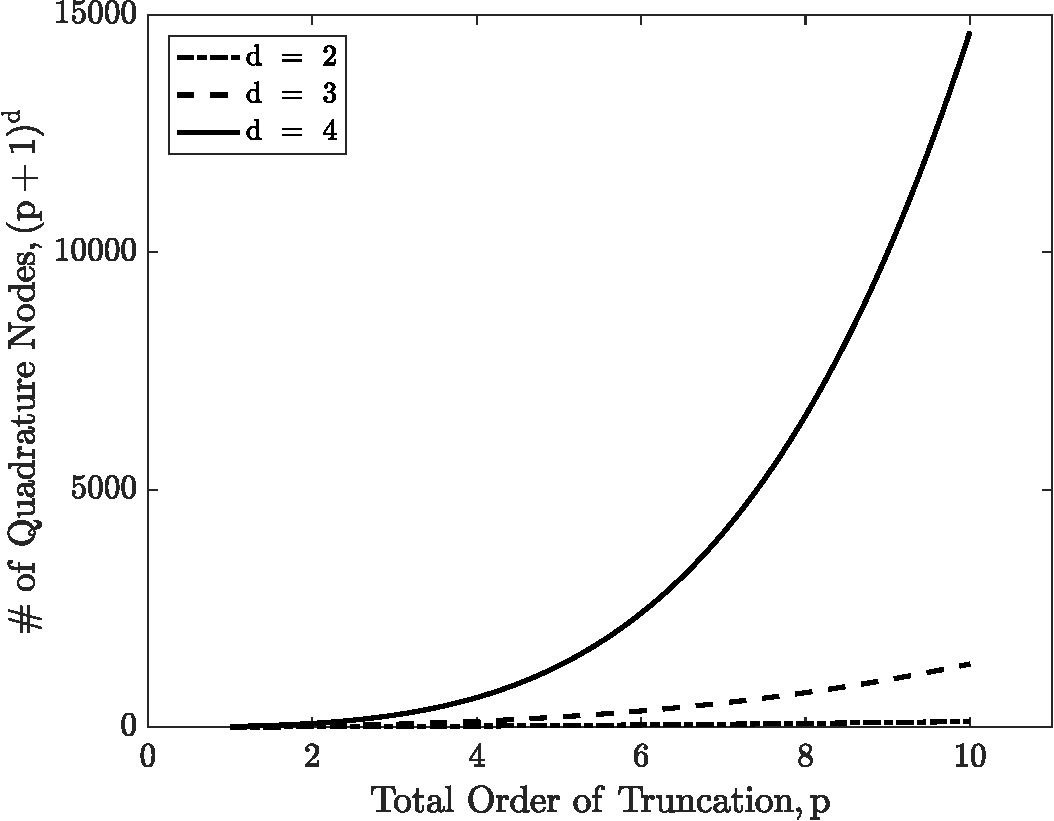
\includegraphics[width=0.70\textwidth]{./Figures/curse}
\caption{Number of multi-dimensional Gauss quadrature nodes, $(p+1)^d$ is plotted against the PCE
 total order truncation, $p$ for 2, 3, and 4 dimensional polynomial basis functions.}
\label{fig:curse}
\end{center}
\end{figure}




